\documentclass[UTF8]{ctexbeamer}
\usetheme{Madrid}
%\usecolortheme{beaver}
\usepackage{graphicx}
\usepackage{multicol}
\usepackage{subfigure}
\DeclareGraphicsExtensions{.eps,.ps,.jpg,.bmp,.png}
%%Information to be included in the title page:
%\title{X}
%\author{Deli}
%%\institute{Deli institute}
%\date{\today}
\title[眼睛] %optional
{眼睛}
% [] {} 两个还是有区别的,具体的差异尝试编译一下就了解了。

\subtitle{第九章}
% 副标题,beamer的默认模板中基本上这些内容都有

\author[]{徐骄阳} % (optional, for multiple authors)
% {Deli1\inst{1} \and Deli2\inst{2}}

\institute[系统科学学院]{系统科学学院} % (optional)
% {
% 	\inst{1}%
% 	Faculty of Physics\\
% 	Very Famous University
% 	\and
% 	\inst{2}%
% 	Faculty of Chemistry\\
% 	Very Famous University
% }

\date[\today]{} % (optional)
%在每个section 前边单独插入当前章节高亮的目录页(当然最原始的目录页你还是需要手动录入的,不要想偷懒)
\AtBeginSection[]
{   
    \begin{frame}
        \frametitle{目录}
        \begin{multicols}{2}    
            \tableofcontents[currentsection,hideallsubsections]
        \end{multicols}
    \end{frame}

	% \begin{frame}
	% 	\frametitle{梗概}
	% 	\tableofcontents[hideallsubsections]
	% \end{frame}
}
\begin{document}
\frame{\titlepage}
\section*{引言}
\begin{frame}
    \frametitle{引言}

    \textbf{视觉}(vision)对于动物而言非常重要,因为它赋予了生命感知周围物体的一个途径。
    一个智能体通过视觉便能接收光信号进行检测与辨识,经过大脑的加工,对环境的变化做出相应的响应。

    哺乳动物的视觉系统始于眼睛,眼睛的背部是\textbf{视网膜}(retina)这里拥有特化的,将光能转化为神经活动的光感受器。
    眼睛的其余部分类似于相机的光学原理,在视网膜上形成清晰的,但暂时的图像。此外眼睛还有自动调节亮度差异,自动聚焦感兴趣物体,移动目标跟踪
    以及通过眼泪和眨眼保持表面的清洁。
    
    此处强调视网膜与胶卷有很大的不同,每个眼睛都有两个互相重叠的视网膜:一个特化为在低亮度(黄昏至黎明)时段工作;
    另一个特化为高亮度时工作,视网膜的输出会进行一定的处理与且与光的绝对强度无关。

    视网膜神经元的轴突汇聚成视神经,它们以动作电位的方式将视觉信息传送至数个履行各种功能的大脑结构趋于、
    视神经的一些中枢靶结构参与一些与昼夜节律同步的生物节律的调节,另外一些则参与对眼睛位置和光学功能的控制。
    然而视觉通路肿第一个突触中继站是位于丘脑背侧的一个细胞群体,叫做\textbf{外侧膝状体核}(lateral geniculate nucleus, LGN)
    视觉信息自LGN传至大脑皮层,进而得到解读和记忆。
\end{frame}
\section{光的特性}
\subsection{光}
\subsection{光学}
\begin{frame}
    \frametitle{光}
    \scriptsize{光是眼睛所能看见的电磁辐射。电磁辐射可以被描述为能量波。与其他波一样,电磁波具有\textbf{波长}(相邻波峰或波谷的间距);\textbf{频率}(每秒波的个数);\textbf{幅度}(波峰波谷的差距)。}
    \begin{figure}
        \centering
        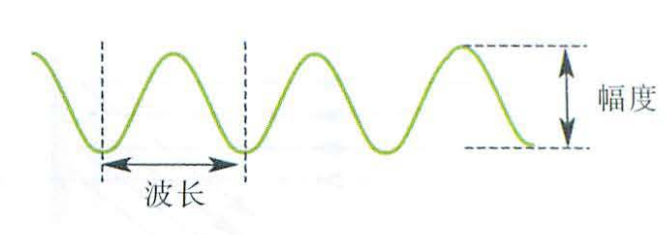
\includegraphics[height=0.2\textheight]{img/sec1-1.png}
        \caption{电磁波的特点\label{sec1-1}}
    \end{figure}
    \begin{figure}
        \centering
        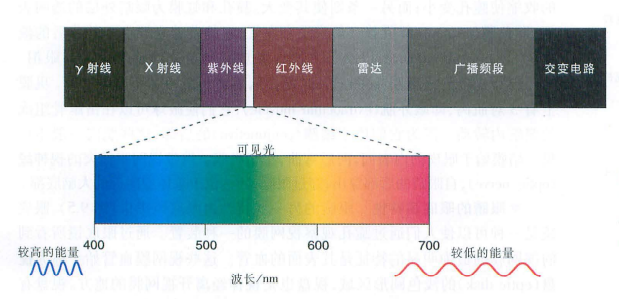
\includegraphics[height=.3\textheight]{img/sec1-2.png}
        \caption{电磁频谱\label{sec1-2}}
    \end{figure}
    电磁辐射的能量的容纳是和它的频率成正比,与波长呈反比。
\end{frame}

\subsection{光学}
\begin{frame}
    \frametitle{光学}

    \begin{columns}
            \column{.6\textwidth}{
            在真空中,电磁辐射波沿直线传播。在大气中光也可近似为直线传播,
            直到光与物体表面的原子或者分子发生交互作用。这些相互作用包括反射、吸收和折射。
            \begin{itemize}
                \item 反射是光线在物体表面的反弹。例如镜子的反光。
                \item 吸收是光能在粒子或者表面的转换。例如光能转换为热能。
                \item 折射是光通过介质分界面的弯折。眼睛中的图像通过光的\textbf{折射}到达视网膜。
            \end{itemize}
        }
        \column{.4\textwidth}{
            \begin{figure}
                \centering
                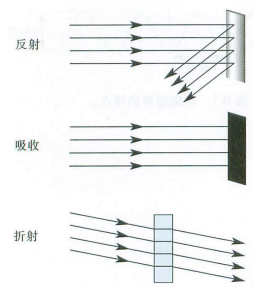
\includegraphics[width=.8\textwidth]{img/sec1-3.png}
                \caption{光与环境的相互作用\label{sec1-3}}
            \end{figure}
        }
    \end{columns}

\end{frame}

\section{眼睛的结构}
\subsection{大体解剖结构}
\subsubsection*{眼底镜特性}
\subsection{横切面解剖结构}
\section{眼睛中图像的形成}
\subsection{角膜的折射}
\begin{frame}
    \frametitle{眼睛中图像的形成}

    眼睛接收环境中由物体发射或反射的光线,并将他们聚焦于视网膜以成像。光在穿过角膜弯曲的表面时候
    会发生偏折。自折射表面至平行光的汇聚点的距离称为\textbf{焦距}焦距和角膜的曲率有关;弯曲程度

\end{frame}
\subsection{晶状体的适应性调节}
\subsection{瞳孔对光反射}
\subsection{视野}
\subsection{视锐度}

\section{视网膜的显微解剖}
\begin{frame}
    \frametitle{视网膜结构}

    \begin{columns}
        \column{0.5\textwidth}{
        下面介绍光能转化为神经活动的过程。先介绍视网膜细胞结构,
        以便大致了解图像处理过程。

        如图\ref{pic4-1},光信息自色素吸收后通过光感受器经双极细胞传导至神经节细胞,
        神经节细胞的轴突汇聚成视神经离开眼球。水平细胞和无长突细胞通过侧向联系调节双极细胞和神经节细胞。
        }
        \column{0.5\textwidth}{
            \begin{figure}
                \centering
                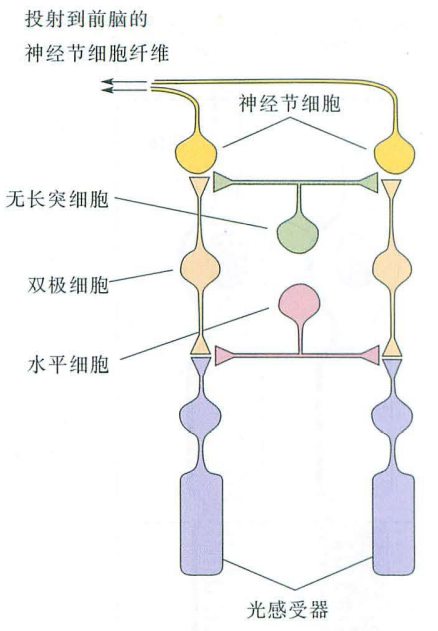
\includegraphics[width=0.6\textwidth]{img/pic4-1.png}

                \caption[]{{视网膜信息处理系统}\label{pic4-1}}
            \end{figure}
        }
    \end{columns}

\end{frame}
\subsection{视网膜的分层组构}
\begin{frame}
    \frametitle{视网膜分层组构}

    \begin{columns}
        \column{.5\textwidth}{
            注意到,光必须穿过几个细胞层才能到达位于视网膜后端的光感受器细胞。视网膜按相对眼球中央的位置由里到外命名:
            \scriptsize{
            \begin{itemize}
                \item \textbf{神经节细胞层}(ganglion cell layer),包含神经节细胞的胞体
                \item \textbf{内核层}(inner nuclear layer),含有双极细胞,水平细胞和无长突细胞的胞体
                \item \textbf{外核层}(outer nuclear layer),含有光感受器胞体
                \item \textbf{光感受器外段层}(layer of photoreceptor outer segments)
            \end{itemize}
            }
        }
        \column{.5\textwidth}{
            \begin{figure}
                \centering
                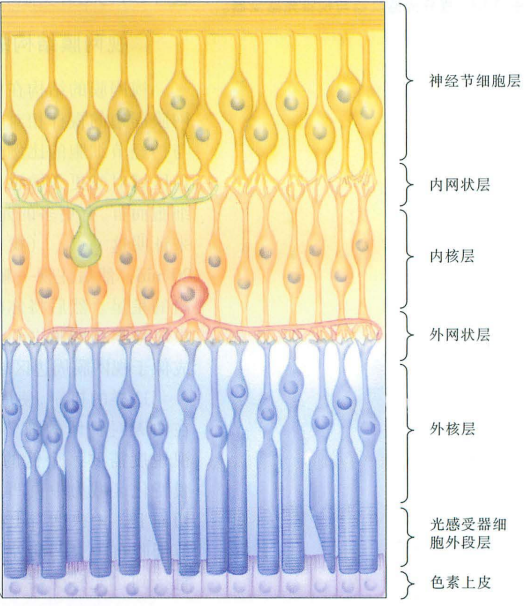
\includegraphics[height=.7\textheight]{img/pic4-2.png}
                \caption{视网膜的分层组构\label{pic4-2}}
            \end{figure}
        }
    \end{columns}

\end{frame}

\subsection{光感受器的结构}
\begin{frame}
    \frametitle{光感受器结构}

    \begin{columns}
        \column{.6\textwidth}{
            光辐射与神经信号的转换发生在视网膜后部的1.25亿个光感受器中。每个光感受器由外段、内段、胞体和突触终末组成。
            \textbf{外段}含有大量膜盘(membranous disk),其上存在光敏感的视色素对光进行吸收,触发光感受器膜电位的变化。
            根据外段外形不同分为:
            \scriptsize{
                \begin{itemize}
                    \item \textbf{视杆光感受器}(rod photorecptor):具有较长的桶状外段,其中含有大量膜盘,不同视杆色素无差异
                    \item \textbf{视锥光感受器}(cone photorecptor):具有较短锥形外段,含有膜盘数较少但色素密度高且存在三种色素类型
                \end{itemize}
            }
            这导致了视网膜的双重性:暗视视网膜只是用视杆,明视视网膜主要使用视锥。视色素差异导致各种视锥对不同波长的光敏感,即仅由视锥对色觉有贡献。
        }
        \column{.4\textwidth}{
            \begin{figure}
                \centering
                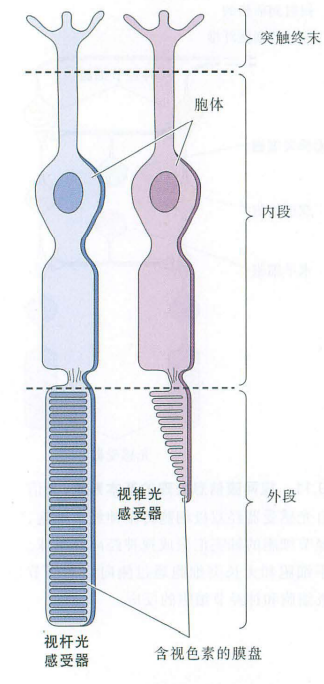
\includegraphics[width=.5\textwidth]{img/pic4-3.png}
                \caption{视杆与视锥光感受器\label{pic4-3}}
            \end{figure}
        }
    \end{columns}

\end{frame}


\subsection{视网膜结构的区域差异}

\begin{frame}
    \frametitle{视网膜结构的区域差异}
    
    \begin{columns}
        \column{.5\textwidth}{
            视网膜的结构在中央凹和视网膜的周边是有所不同的。其细胞分布如图\ref{pic4-4}(a),
            视锥主要集中在视网膜的中心,视杆细胞主要分布于周边视网膜,中央凹内没有视杆细胞。

            由结构图\ref{pic4-4}(b),在视网膜中心由较少的光感受器细胞直接向一个神经节细胞提供信息;在周边视网膜则较多。
            这一结构安排使得周边视网膜对暗淡光线的检测更为有利,而中心视网膜则对提高视觉精度更为有利。
        }
        \column{.5\textwidth}{
            \begin{figure}
                \centering
                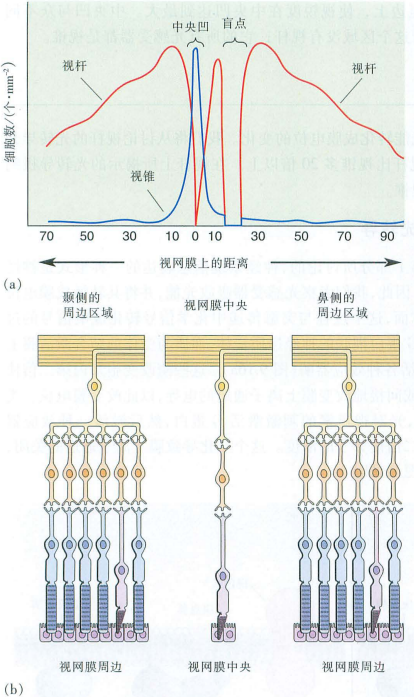
\includegraphics[height=.7\textheight]{img/pic4-4.png}
                \caption{视网膜细胞分布的区域差异\label{pic4-4}}
            \end{figure}
        }
    \end{columns}

\end{frame}
\begin{frame}
    \frametitle{视网体结构汇总}
    \begin{figure}
        \centering
        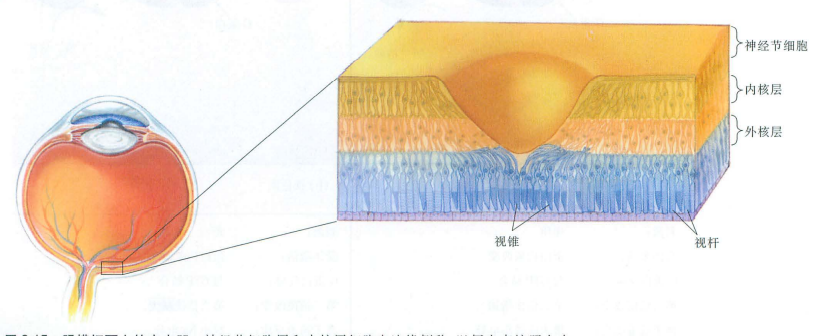
\includegraphics[width=.8\textwidth]{img/pic4-5.png}
        \caption{视网膜显微结构\label{pic4-5}}
    \end{figure}
    \tiny{Tip:图中神经节细胞层和内核层细胞向边缘侧移,以便光直接照在中央凹的光感受器上,提高中央区域的视锐度,同时也提升了周边视网膜的光敏感性。}

\end{frame}

\section{光传导}
\subsection{视杆中的光传导}
\subsection{视锥中的光传导}
\subsection{暗适应和明适应}
\section{视网膜的信息处理}
\subsection{外网状层的信息传递}
\begin{frame}
    \frametitle{外网状层的信息传递\label{frame1}}

    光感受器在在\textbf{黑暗环境下去极化},并释放神经递质(据认为是谷氨酸)。

    在外网状层,每个光感受器都和两种视神经元:双极细胞和水平细胞形成突触。
    其中,双极细胞构成自感受器到神经节细胞的直接通路。
    水平细胞负责外网状层信息的侧向传递,以影响其临近的双极细胞的活动性。

    基于对神经递质的反应,双极细胞分为两类:
    \begin{itemize}
        \item \textbf{撤光双极细胞}(OFF bipolar cell)谷氨酸门控阳离子通道通过$Na^+$的内流,介导经典的去极化的兴奋性突触。
        \item \textbf{给光双极细胞}(ON bipolar cell)对谷氨酸的响应为超极化。
    \end{itemize}
    OFF和ON的定义在于这些细胞是否对撤光(更多谷氨酸)或给光(少谷氨酸)产生去极化影响。
    双极细胞的\textbf{感受野}(receptive field)是视网膜上给光刺激能改变细胞膜电位的区域。
    
\end{frame}

\begin{frame}
    \frametitle{双极细胞的感受野}

    \begin{columns}
        \column{.5\textwidth}{
            双极细胞的感受野由两部分组成:
            \begin{itemize}
                \item 一个提供直接光感受器输入的圆形视网膜区域,称为感受野中心。
                \item 以及一个通过水平细胞提供输入的视网膜的环形区域,称为感受野周边。
            \end{itemize}
            感受野越靠近中心越小,越靠近周边越大。
        }\column{.5\textwidth}{
            \begin{figure}
                \centering
                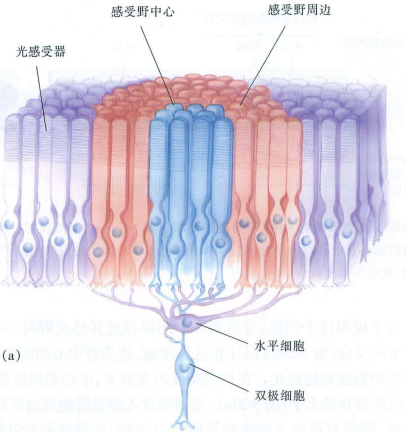
\includegraphics[width=.8\textwidth]{img/pic6-1.png}
                \caption{细胞连接示意图\label{pic6-1}}
            \end{figure}
        }
    \end{columns}

\end{frame}

\begin{frame}
    \frametitle{信号传递通路}

    \begin{columns}
        \column{0.5\textwidth}{
            在感受野中心的光通过直接通路给光中心型的双极细胞\textbf{去极化};
            在感受野周边的光通过简介通路给光中心型双极细胞\textbf{超极化}。

            由于水平细胞的介入,光对周边光感受器的作用总是与其对中心光感受器的作用相反。
            我们称这些细胞具有颉颃的\textbf{中心-周边感受野}
        }\column{.5\textwidth}{
            \begin{figure}
                \centering
                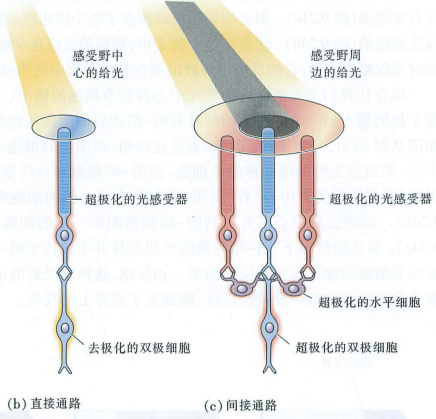
\includegraphics[width=\textwidth]{img/pic6-2.png}
                \caption{直接通路与间接通路\label{pic6-2}}
            \end{figure}
        }
    \end{columns}
    \scriptsize{Tip:图\ref{pic6-2}仅仅是幻灯片\ref{frame1}提到双极细胞的一种,
    另一种的去/超极化过程与其相反。}

\end{frame}



\section{视网膜的输出}

\subsection{神经细胞感受野}
\begin{frame}
    \frametitle{神经节细胞的感受野}
    % \begin{columns}
        % \column{.5\textwidth}{
            中心-周边感受野的组织方式从双极细胞通过内网状层的突触传向神经节细胞。
            内网状层的无长突细胞的侧向链接也参与神经节细胞感受野的形成,但至今我们对这些连接的具体作用知之甚少。
        
            多数神经节细胞具有和上述双极细胞一样的同心圆式的中心-周边感受野结构。给光中心和撤光中心神经节细胞接收同类双极细胞的输入。
        
            多数视网膜神经节细胞对同时覆盖其感受野中心和周边的光刺激变化并无反应,主要对他们感受野内的\textbf{亮度差异}有反应。        
        % }\column{.5\textwidth}{
            \begin{figure}
                \centering
                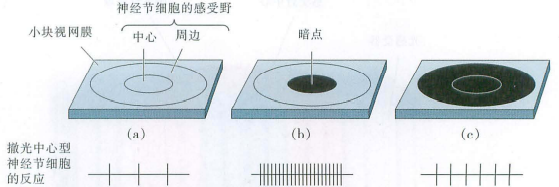
\includegraphics[width=.8\textwidth]{img/pic7-1.png}
                \caption{神经节细胞的中心-周边感受野\label{pic7-1}}
            \end{figure}
            \tiny{
                当一个暗点投射在撤光中心型神经节细胞的感受野中心时,细胞发放一串动作电位,但暗点范围扩大,则放电大幅减少。
            }
        % }
    % \end{columns}
    
\end{frame}

\begin{frame}
    \frametitle{神经节细胞感受野对明暗边界的调制}
    考察明暗边界对撤光中心神经节细胞输出的影响。根据实验,该信号有如图\ref{pic7-2}所示反应。%#TODO:做个图像分析
    \begin{figure}
        \centering
        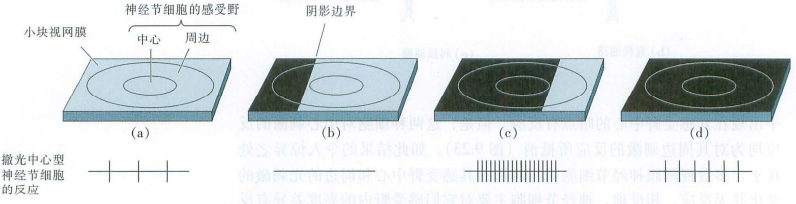
\includegraphics[width=.8\textwidth]{img/pic7-2.png}
        \caption{神经节细胞对感受野内明暗边界的反应\label{pic7-2}}
    \end{figure}
    从神经节细胞感受野的组织形式,我们可以推断,世界系统特化为对局部空间变化进行检测,而不是对于落在视网膜上光的绝对幅度进行检测,因此,\textbf{视网膜对光或暗的感知是相对的}。
\end{frame}
\subsection{神经细胞的类型}
\begin{frame}
    \frametitle{神经细胞按大小分类}

    在哺乳类视网膜,多数数神经节细胞具有一个中心-周边感受野,其中心区域或具给光反应或具撤光反应。他们可以进一步根据外形、突触连接、和
电生理特性进行分类。

在恒河猴和人体视网膜,已经发现两种主要 神经细胞:
    \scriptsize{
        \begin{itemize}
            \item 一种是大的\textbf{M型神经节细胞}(M-type ganglion cell),占神经节细胞总数的5\%;
            \item 另一种为小的\textbf{P型神经节细胞}(P-type ganglion cell),占神经节细胞总数的90\%;
            \item 其余的非M-非P细胞占5\%。
        \end{itemize}
    }

    M细胞具有较大的感受野,传导动作电位速度快,低对比度刺激更敏感。
    此外始于M细胞感受野中心的刺激为瞬时动作电位的发放,
    而对于P细胞则为和刺激时间等长的持续放电,如图\ref{pic7-3}。
    一种观点认为:M细胞对移动刺激的检测具有重要意义,而P细胞对刺激的形状及席位之处更敏感。
    \begin{figure}
        \centering
        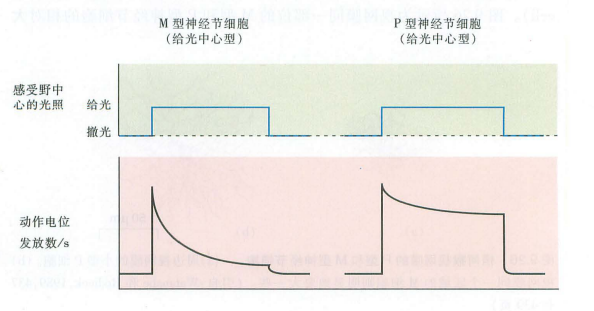
\includegraphics[height=.3\textheight]{img/pic7-3.png}
        \caption{M型和P型神经细胞的对光反应\label{pic7-3}}
    \end{figure}

\end{frame}
\begin{frame}
    \frametitle{神经细胞按颜色敏感性分类}

    视网膜神经节细胞间另一个差异在于P细胞和一些非M非P细胞对光的波长的敏感性差异。
    这些颜色敏感神经元的大部分称为\textbf{颜色对立细胞},
    反映了这种细胞的感受野中心对一种波长的反应可以为出现在感受野周边区域的另一种波长的光所抵消的事实。
    在P细胞,相互对立的颜色为蓝色和黄色。如图\ref{pic7-4},考虑红色给光中心和绿色撤光周边反应的细胞。
    %#TODO:没太看懂↑
    \begin{figure}
        \centering
        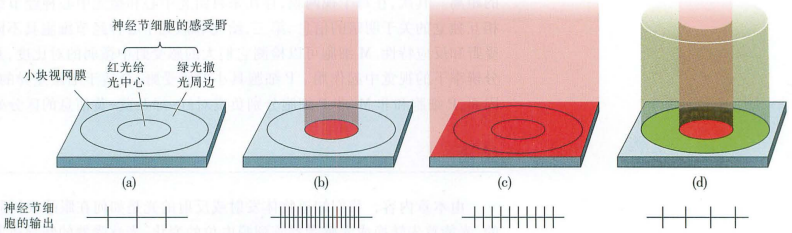
\includegraphics[width=.8\textwidth]{img/pic7-4.png}
        \caption{P型神经节细胞颜色对立的中心-周边感受野\label{pic7-4}}
    \end{figure}


\end{frame}

\subsection{并行处理}
\begin{frame}
    \frametitle{视觉系统的并行处理与信息整合需求概述}
    \begin{itemize}
        \item 由于我们是用两只眼睛看世界的,便产生了两个并行的信息流,在中枢系统中,这些信息流通过比较给出了关于深度(距离)的信息。
        \item 其次在每个视网膜,存在来自给光中心和撤光中心神经节细胞具有不同的感受野和反应特性,
        M细胞可以检测他们大的感受野中微弱的对比度,并在低分辨率下的视觉中起作用。
        P细胞据哟u小的感受野,合适于席位差异的检测。
        因此,P细胞和非M-非P细胞分别负责对红-绿及红-蓝信息的区分处理。
    \end{itemize}
    

\end{frame}

\section*{结语}
\begin{frame}
    \frametitle{结语}

    bbb

\end{frame}
\end{document}